% ----
% COMP1204 CW1 Report Document
% ----
\documentclass[]{article}
\usepackage{xcolor}
\usepackage{listings}
\lstset{basicstyle=\ttfamily,
  showstringspaces=false,
  commentstyle=\color{red},
  keywordstyle=\color{blue},
  breaklines=true,
  stringstyle=\color{purple}
}
\usepackage{graphicx}
\graphicspath{ {./images/} }

% Reduce the margin size, as they're quite big by default
\usepackage[margin=1in]{geometry}

\title{COMP1204: Data Management \\ Coursework One: Hurricane Monitoring }
% Update these!
\author{Orasiki Wellington \\ oew1g21}

% Actually start the report content
\begin{document}

% Add title, author and date info
\maketitle

\section{Introduction}
\paragraph{}The aim of this report is to analyse a bash script which data cleans hurricane monitoring data. This script will generate a CSV (comma-separated values) file when given a KML (Keyhole Markup Language) file.  The CSV file contains relevant information from the KML file and is used to generate storm plots. This will be seen in practise when 3 example KML files are passed into the bash script to generate 3 different CSV files and in turn, 3 different storm plots.



\section{Create CSV Script}

\subsection{Script}

\lstinputlisting[language=Bash, caption = Bash Script Code]{create_csv.sh}

\subsection{Overall Explanation}

\paragraph{}In total, the bash script consists of 6 programs joined together using pipes. These programs will be explained in detail with the first line of the script.

\begin{lstlisting}[language=Bash, caption = First line of Bash script]
#!/bin/bash
\end{lstlisting}
\paragraph{}The first line of the bash script indicates to the system's operating system to call on the bash shell to run the commands that come after it in the script.

\begin{lstlisting}[language=Bash, caption = First program]
awk -F "</*td>|</*tr>" '/<td>.*/ {print $3}' "$1" 
\end{lstlisting}
\paragraph{}The first program retrieves the kml file passed as the first argument of the script. It uses the awk command with the -F option to tell awk that the field separators are the closing and opening td or tr tags in the file. This is easily done using wildcards. Next, the program fetches all records containing td tags and prints the third field. This returns the contents between the td tags. The output of this program is piped to the second program which is a sed program.

\begin{lstlisting}[language=Bash, caption = Second program]
sed -e 's/\(.<B>\|<\/B>.\|;.*\)//g' -e '/hr/d' -e's/\(, \)/,/g'
\end{lstlisting}
\paragraph{}The second program is a sed program that works on the output of the first program. The sed program is used with the -e option which tells sed to execute the command line arguments after this as a sed program. 
\paragraph{}The sed program has many functions. One function of the sed program is to remove all lines containing the hr tag. Another function of the sed program is to remove the B opening and closing tags and everything that comes after a semi colon in all line. Lastly, the sed program removes all spaces after a comma. The last two deletions the sed program performs are inline and is done via global substitution with the help of wildcards. This differs from the first case mentioned which deletes the whole line rather than words in a line. The output of the sed program is piped to the third program; another awk program.

\begin{lstlisting}[language=Bash, caption = Third program]
awk '(NR%2==0) {print}'
\end{lstlisting}
\paragraph{}The third program is an awk program that receives output from the second program. It only prints records that are divisible by 2. This is done, to remove td tags that don't contain the information we need. The output of this program is piped to the fourth program.

\begin{lstlisting}[language=Bash, caption = Fourth program]
awk '{line=line "," $0}  (NR%4==0) {print substr(line,2); line=""}'>"$2" 
\end{lstlisting}
\paragraph{}The main function of the fourth program is to concatenate the records of the output it receives from the third program. The program is an awk program which initialises a variable called line and adds the current record to the variable. The lines are separated using a comma. The program concatenates the first four records then re-initialises the line variable to null and the loop begins again. The output of this program is written to the file which is passed as the second argument of the script before being piped to the fifth program.

\begin{lstlisting}[language=Bash, caption = Fifth program]
sed -i '1 i\Timestamp,Latitude,Longitude,MinSeaLevelPressure,MaxIntensity' "$2"
\end{lstlisting}
\paragraph{}The last program is a sed program. It takes the output of the fourth program and inserts the text provided at the first line. The result of this is written to the file which is passed as the second argument of the bash script.


\section{Storm Plots}

\begin{figure}
    \centering
    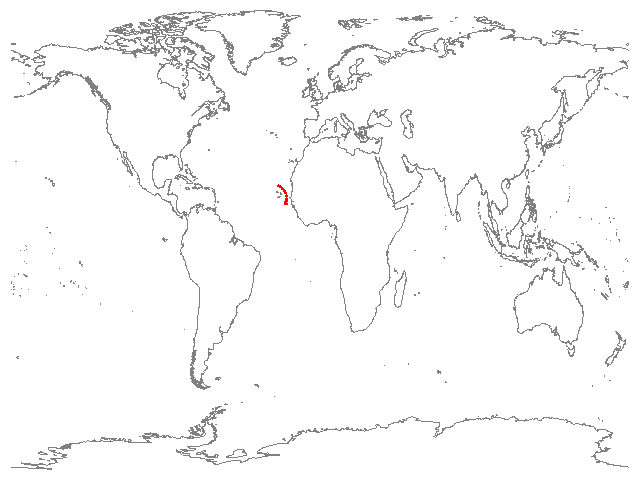
\includegraphics[width=\textwidth]{cw1_material/images/storm_plot0.png}
    \caption{Storm plot diagram produced from the al102020.kml file}
    \label{fig:storm_plot1}
\end{figure}

\begin{figure}
    \centering
    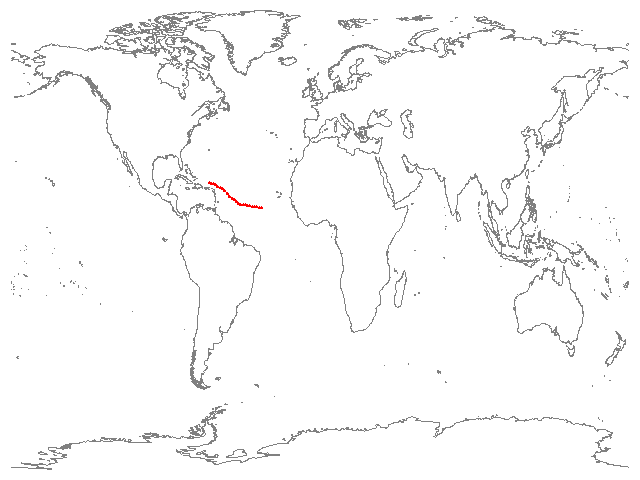
\includegraphics[width=\textwidth]{cw1_material/images/storm_plot1.png}
    \caption{Storm plot diagram produced from the al112020.kml file}
    \label{fig:storm_plot2}
\end{figure}

\begin{figure}
    \centering
    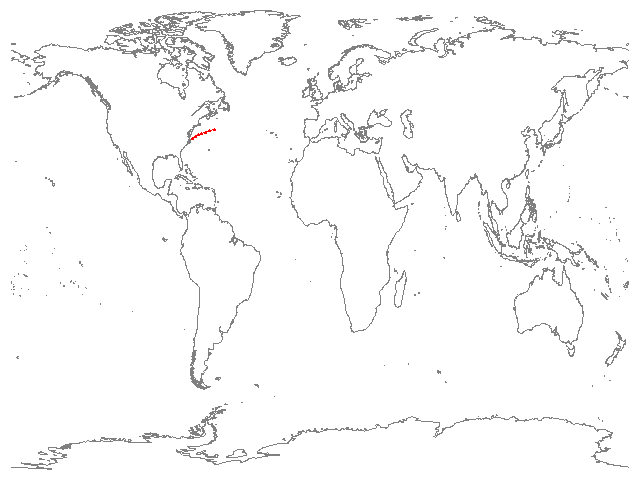
\includegraphics[width=\textwidth]{cw1_material/images/storm_plot2.png}
    \caption{Storm plot diagram produced from the al122020.kml file}
    \label{fig:storm_plot3}
\end{figure}
\end{document}
